\chapter{Landasan Teori}
\label{chap:definition}

\section{Tahap Data Mining}
Proses pada \textsl{data mining} dapat dibagi menjadi beberapa tahap seperti pada gambar 2.1

\begin{figure}
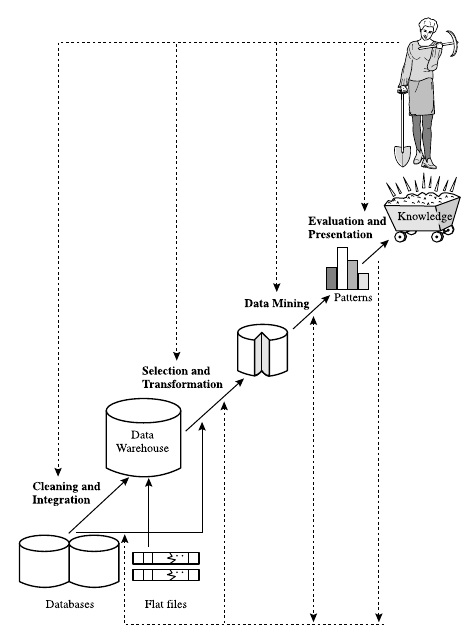
\includegraphics[scale=1]{Gambar/tahapdatamining.jpg}
\caption[Tahap \textsl{Data Mining}, Sumber Data Mining Concepts & Techniques]{Tahap \textsl{Data Mining}, Sumber Data Mining Concepts & Techniques} 
\end{figure}

Terdapat 7 tahap pada \textsl{data mining}:
\begin{itemize}
	\item \textsl{Data cleaning}
	\item \textsl{Data integration}
	\item \textsl{Data selection}
	\item \textsl{Data transformation}
	\item \textsl{Data mining}
	\item \textsl{Pattern Evaluation}
	\item \textsl{Knowledge presentation}
\end{itemize}

\section{\textsl{Data cleaning}}
\textsl{Data cleaning} merupakan tahap \textsl{data mining} untuk menghilangkan \textsl{missing value} dan \textsl{noisy data}. Pada umumnya, \textsl{data} yang diperoleh dari \textsl{database} terdapat nilai yang tidak sempurna seperti nilai yang hilang, nilai yang tidak \textsl{valid} atau bahkan salah ketik. Nilai-nilai tersebut dapat diatasi dengan cara \textsl{smoothing techniques}. Atribut dari suatu \textsl{database} yang tidak relevan atau redudansi bisa diatasi dengan menghapus atribut tersebut. 

\section{\textsl{Data integration}}


\section{\textsl{Data selection}}
\section{\textsl{Data transformation}}
\section{\textsl{Data mining}}
\section{\textsl{Pattern Evaluation}}
\section{\textsl{Knowledge presentation}}

\section{\textsl{Spatial and spatiotemporal}}